\documentclass[conference]{IEEEtran}
\usepackage{amsmath,amssymb}
\usepackage{graphicx}
\usepackage{booktabs}
\usepackage{multirow}
\usepackage{array}
\usepackage{url}
\usepackage{cite}
\usepackage{float}

\title{Comparative Study of Classical Elman Neural Network (ENN), Quantum Elman Neural Network (QENN) Using Qiskit, and Quantum Elman Neural Network (QENN) Implemented in Microsoft Q\# for Stock Closing Price Prediction}

\author{
\IEEEauthorblockN{Reproduction and Extension Study}
\IEEEauthorblockA{Implementation stacks: PyTorch, Qiskit/Qiskit-Aer, Microsoft Q\# (Python interop)}
}

\begin{document}
\maketitle

\begin{abstract}
This paper presents a complete reproduction and extension study of Liu and Ma's Quantum Elman Neural Network (QENN) for stock closing price prediction \cite{ref43}. The reproduction follows the original mathematical framework and extends it with two independent quantum software-stack realizations: QENN-Qiskit (IBM Qiskit/Qiskit-Aer) and QENN-Q\# (Microsoft Q\# with Python interop and faithful NumPy fallback). A comparative evaluation is conducted on six stock-index datasets with chronological 80/20 train-test split, window size 6, global min-max normalization to $[-1,1]$, and normalized mean squared error (NMSE) as the metric (lower is better). All reported results are 10-run averages over seeds 0--9. The study provides explicit cross-stack portability analysis, quantitative gap analysis against paper-reported QENN values, smoke-test gating, and full reproducibility controls. The reproduced classical ENN baselines achieve the lowest NMSE in this software-simulation regime, while QENN-Q\# reproduces paper-reported QENN values more closely than QENN-Qiskit on most datasets. The paper also confirms bounded adaptive learning-rate behavior under DCQGA and analyzes implementation-level causes of long-horizon divergence despite amplitude-level equivalence checks.
\end{abstract}

\begin{IEEEkeywords}
Stock closing price prediction, Elman neural network, quantum neural network, Qiskit, Q\#, DCQGA, NMSE, reproducibility.
\end{IEEEkeywords}

\section{Introduction}
Stock market forecasting is a high-impact but difficult time-series problem because market dynamics are nonlinear, nonstationary, volatility-driven, and influenced by macroeconomic, political, and social factors \cite{ref14,ref37,ref38}. Long-range dependencies and regime shifts further complicate model design and optimization. As a result, robust low-error forecasting remains challenging even for modern machine learning methods.

Classical forecasting literature includes ARIMA-hybrid approaches \cite{ref2,ref37}, neuro-fuzzy systems \cite{ref1,ref4,ref8}, GMDH-type neural models \cite{ref22,ref23,ref24,ref30}, and broader ANN families \cite{ref10,ref12,ref25}. These approaches deliver useful practical performance, but common limitations remain: difficult nonconvex optimization, local-minima sensitivity, distribution-shift fragility, and convergence-speed bottlenecks in highly nonlinear settings.

Quantum computing introduces a complementary representational paradigm via linear superposition, where an $n$-qubit system spans a $2^n$-dimensional Hilbert space \cite{ref3,ref16,ref18,ref21,ref28}. QNN formulations are therefore motivated by potential advantages such as exponential storage capacity, compact structure, improved stability, parallel state processing, and reduced catastrophic forgetting risk under suitable modeling assumptions.

Liu and Ma \cite{ref43} proposed the Quantum Elman Neural Network (QENN), combining ENN-style recurrence and context memory with quantum-state-inspired hidden/output layers and a Double Chains Quantum Genetic Algorithm (DCQGA) for adaptive learning-rate tuning. Their framework was validated on six stock-index datasets and provides a rigorous starting point for reproducible cross-implementation studies.

This paper makes five explicit contributions:
\begin{enumerate}
\item \textbf{Faithful QENN framework reproduction:} recurrence-aware architecture, self-connected context update (gain $c=0.5$), and per-epoch DCQGA tuning of bounded $(\eta_1,\eta_2,\eta_3)$.
\item \textbf{QENN-Qiskit:} QENN implemented with IBM Qiskit/Qiskit-Aer statevector simulation, with analytical equivalence checks against $f_0(x)=\cos(e^x)$ and $f_1(x)=\sin(e^x)$.
\item \textbf{QENN-Q\#:} QENN implemented via Microsoft Q\# interop (\texttt{QENN.GetAmplitudes}) with faithful NumPy fallback when Q\# runtime is unavailable, with explicit execution-mode labeling.
\item \textbf{Quantitative gap analysis:} absolute/relative per-dataset gaps between reproduced quantum variants and paper-reported QENN values (Table~\ref{tab4}).
\item \textbf{Reproducibility controls:} seeds 0--9, smoke-test gating, chronological split (no shuffle), and fixed sliding-window size 6.
\end{enumerate}

Scope: classical ENN uses PyTorch \texttt{nn.RNN} (\texttt{tanh}), Xavier initialization, SGD ($lr=0.01$), hidden widths $\{10,20,40,70,100\}$; QENN uses $6\times5\times1$ in all quantum experiments. Section~II presents theory, Section~III details QENN and DCQGA, Section~IV reports experiments and discussion, and Section~V concludes.

\section{Preliminary Theory}
\subsection{Architecture of Elman Neural Network}
The Elman Neural Network (ENN) is globally feedforward and locally recurrent, with input, hidden, context, and output layers. The context layer acts as a one-step delay memory. Its core equations are:
\begin{align}
u(k) &= f\!\left(w_1\cdot u_x(k) + w_2\cdot x(k-1)\right), \label{eq1}\\
u_x(k) &= u(k-1), \label{eq2}\\
y(k) &= g\!\left(w_3\cdot u(k)\right). \label{eq3}
\end{align}
Here $x$ is input, $u$ hidden output, $u_x$ context output, $y$ model output; $w_1,w_2,w_3$ are context-to-hidden, input-to-hidden, and hidden-to-output weights; $f$ and $g$ are activations.

Implementation details: PyTorch \texttt{nn.RNN} (\texttt{nonlinearity='tanh'}, \texttt{batch\_first=True}), Xavier-uniform initialization for all weights, zero biases, linear output layer with Xavier-uniform weights, SGD optimizer ($lr=0.01$), and 100 epochs. Recurrence is implemented statelessly across the full ordered sequence each epoch with zero initial hidden state. Hidden widths are $\{10,20,40,70,100\}$, each run 10 times; NMSE is averaged.

\begin{figure}[t]
\centering
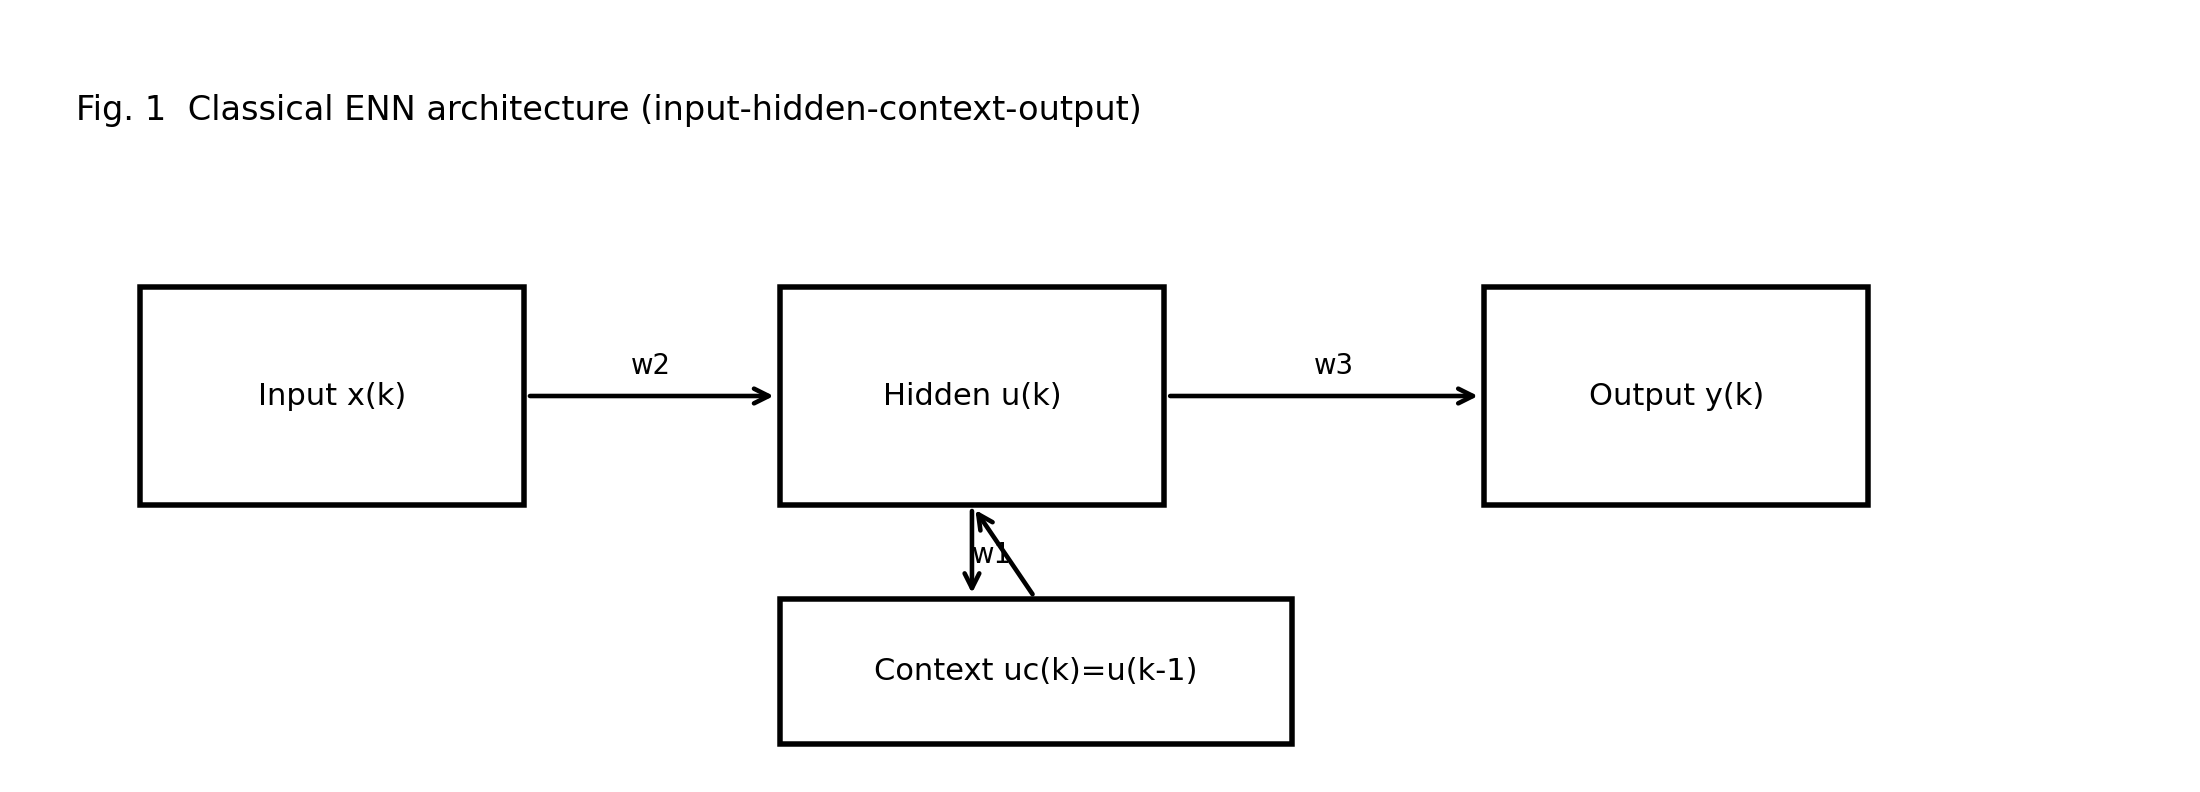
\includegraphics[width=\columnwidth]{fig1_enn_schematic.png}
\caption{Classical ENN block diagram: Input $x(k)\rightarrow$ Hidden $u(k)\rightarrow$ Output $y(k)$, with context $u_c(k)=u(k-1)$ feedback to hidden via $w_1$.}
\label{fig1}
\end{figure}

\subsection{Closing Price}
Closing price is the final transaction price for a trading day and is widely used for trend analysis and risk-aware decision support. This study uses daily closing prices from six global stock indices (Section~IV-A).

\subsection{Linear Superposition}
Classical bits are deterministic ($0$ or $1$), whereas a qubit is a superposition:
\begin{equation}
\lvert\phi\rangle = \alpha_0\lvert 0\rangle + \alpha_1\lvert 1\rangle,\quad |\alpha_0|^2+|\alpha_1|^2=1. \label{eq4}
\end{equation}
For $n$ qubits:
\begin{equation}
\lvert\Phi\rangle = \sum_{i=0}^{2^n-1}\alpha_i\lvert i\rangle,\quad \sum_i|\alpha_i|^2=1. \label{eq5}
\end{equation}
The $2^n$-dimensional Hilbert space motivates QENN hidden-state composition via tensor products. Measurement collapses to basis state $\lvert i\rangle$ with probability $|\alpha_i|^2$.

\subsection{Learning Rate Tuning}
Learning-rate choice controls convergence speed and stability: overly large rates may diverge; overly small rates train slowly. Classical schedules (annealing, warmup, cyclical, exponential decay) can be effective but are fixed-policy:
\begin{equation}
\alpha_t = \alpha_0\cdot\beta^t,\;\beta<1. \label{eq6}
\end{equation}
QENN instead adopts DCQGA to tune three rates per epoch under fixed bounds:
\begin{align}
10^{-5}<\eta_1<10^{-4}, \label{eq7}\\
2\times 10^{-5}<\eta_2<10^{-4}, \label{eq8}\\
9\times 10^{-6}<\eta_3<8\times10^{-5}. \label{eq9}
\end{align}

\section{Quantum Elman Neural Network}
\subsection{Architecture of Quantum Elman Neural Network Model}
QENN retains ENN recurrence and replaces classical neurons with quantum-state-inspired units. The network size is fixed at $n_i\times n_h\times n_o=6\times5\times1$.

Input layer:
\begin{equation}
x(k)=(x_1(k),x_2(k),\ldots,x_{n_i}(k)). \label{eq10}
\end{equation}

Hidden layer (qubit $i$):
\begin{align}
\lvert y_i\rangle(k) &= f_0(\eta_i)\lvert 0\rangle + f_1(\eta_i)\lvert 1\rangle, \label{eq11}\\
\eta_i &= x(k)\cdot w_i + b_i + \tilde a(k)\cdot\tilde w_i, \label{eq12}\\
f_0(x)&=\cos(e^x),\quad f_1(x)=\sin(e^x). \label{eq13}
\end{align}
Here $w_i\in\mathbb{R}^{n_i}$, $b_i\in\mathbb{R}$, $\tilde a(k)\in\mathbb{R}^{2^{n_h}}$, and $\tilde w_i\in\mathbb{R}^{2^{n_h}}$.

Combined hidden state:
\begin{equation}
\lvert y_1\rangle(k)\otimes\cdots\otimes\lvert y_{n_h}\rangle(k)=\sum_i\alpha_i(k)\lvert i\rangle. \label{eq14}
\end{equation}
Thus $\alpha(k)\in\mathbb{R}^{32}$ for $n_h=5$.

Self-connected context update:
\begin{equation}
\tilde a_i(k)=\frac{c\cdot\tilde a_i(k-1)+\alpha_i(k-1)}{\left\|c\cdot\tilde a(k-1)+\alpha(k-1)\right\|},\;\;0<c<1. \label{eq15}
\end{equation}
Implementation uses $c=0.5$.

Output layer:
\begin{equation}
\lvert z_l\rangle(k)=f_0(\alpha(k)\cdot v_l+\tilde b_l)\lvert0\rangle + f_1(\alpha(k)\cdot v_l+\tilde b_l)\lvert1\rangle. \label{eq16}
\end{equation}

Prediction mapping:
\begin{align}
p(\eta) &= \sin(e^{\eta})^2, \label{eq17}\\
\hat y &= 2p(\eta_{\text{out}})-1. \label{eq18}
\end{align}

Qiskit path initializes each hidden-qubit state with \texttt{QuantumCircuit.initialize([c0,c1])} using Qiskit-Aer statevector simulation, with equivalence validation against analytical amplitudes at tolerance $10^{-10}$ (8 random checks/run) and cache reuse. Q\# path uses \texttt{QENN.GetAmplitudes(theta: Double)} and falls back to faithful NumPy encoding when Q\# runtime is unavailable.

All weight matrices ($w_{\text{in}},w_{\text{ctx}},v_{\text{out}}$) use Xavier-uniform initialization; biases are zero-initialized.

\subsection{Learning Algorithm}
The optimization objective is NMSE:
\begin{equation}
E=\frac{1}{N}\sum_{k=1}^{N}\left(y_d(k)-\hat y(k)\right)^2. \label{eq19}
\end{equation}

Paper-form gradient updates are:
\begin{align}
\Delta v_{lj} &= -\eta_1\frac{2}{N}(y_d-y)\dot p(\eta_l)\alpha_j(k), \label{eq20}\\
\Delta\tilde w_{iq} &= -\eta_2\frac{2}{N}(y_d-y)\dot p(\tilde\eta_i)\tilde a_q(k), \label{eq21}\\
\Delta w_{ij} &= -\eta_3\frac{2}{N}(y_d-y)\dot p(\tilde\eta_i)x_j(k). \label{eq22}
\end{align}
Bias updates use the same error term and layer derivative. Parameters update via $\theta(k+1)=\theta(k)+\Delta\theta$.

Implementation note for reproducibility: reproduced training uses full chain-rule backpropagation through tensor-product hidden state,
\begin{equation}
\frac{\partial\hat y}{\partial\eta_{h,i}} = 2\dot p(\eta_{\text{out}})\left(\frac{\partial\alpha}{\partial\eta_{h,i}}\cdot v_{\text{out}}\right), \label{eq23}
\end{equation}
with $\dot p(\eta)=\sin(2e^\eta)e^\eta$. This is stricter than local proxy $\dot p(\tilde\eta_i)$ and preserves forward architecture/loss.

Training procedure: (1) prepare data with chronological 80/20 split, (2) initialize QENN $6\times5\times1$ and normalized uniform context (dim 32), (3) per epoch run DCQGA for $(\eta_1,\eta_2,\eta_3)$ then one full gradient pass, (4) evaluate test NMSE after 100 epochs, (5) repeat 10 runs and average.

\subsection{Double Chains Quantum Genetic Algorithm (DCQGA)}
DCQGA optimizes $(\eta_1,\eta_2,\eta_3)$ each epoch.

Initialization:
\begin{equation}
p_i=\begin{bmatrix}\cos(t_{i1})&\cdots&\cos(t_{in})\\ \sin(t_{i1})&\cdots&\sin(t_{in})\end{bmatrix},\quad t_{ij}=2\pi r,\;r\sim U(0,1). \label{eq24}
\end{equation}

Solution-space transformation:
\begin{align}
X^i_{jc}&=\frac{1}{2}\left[b_j(1+a_{ij})+a_j(1-a_{ij})\right], \label{eq25}\\
X^i_{js}&=\frac{1}{2}\left[b_j(1+b_{ij})+a_j(1-b_{ij})\right]. \label{eq26}
\end{align}

Fitness is $-\text{NMSE}$ (maximization equivalent to minimization). In extended mode, fitness uses up to 256 training samples per call.

Rotation gate:
\begin{equation}
U(\Delta\theta)=\begin{bmatrix}\cos\Delta\theta & -\sin\Delta\theta\\ \sin\Delta\theta & \cos\Delta\theta\end{bmatrix}. \label{eq27}
\end{equation}
Direction is $\operatorname{sgn}(A)$ with $A=a_0b_i-b_0a_i$ against global best amplitudes. Magnitude uses numerical-gradient scaling ($\epsilon=10^{-7}$):
\begin{equation}
\Delta\theta_{ij}=\operatorname{sgn}(A)\cdot\Delta\theta_0\cdot\exp\!\left(-\frac{|\nabla f(X_{ij})|-\nabla f_{\min}}{\nabla f_{\max}-\nabla f_{\min}}\right). \label{eq28}
\end{equation}
Mutation applies quantum-NOT gate $X=\begin{bmatrix}0&1\\1&0\end{bmatrix}$ with probability 0.1.

\section{Experimental Investigations and Discussion}
\subsection{Data Selection}
Six datasets of daily closing prices are used. Table~\ref{tab1} reports statistics from actual CSV files loaded in this implementation.

\begin{table*}[t]
\centering
\caption{Dataset statistics (actual loaded CSVs).}
\label{tab1}
\begin{tabular}{llrrr}
\toprule
Short Name & Long Name & Samples & Min & Max \\
\midrule
BSE & Bombay Stock Exchange & 2,948 & 15,175.08 & 61,765.59 \\
NASDAQ & National Association of Securities Dealers Automated Quotation & 3,021 & 2,091.79 & 16,057.44 \\
HSI & Hang Seng Index & 2,957 & 16,250.27 & 33,154.12 \\
SSE & Shanghai Securities Composite Index & 2,913 & 1,950.01 & 5,166.35 \\
Russell2000 & Russell 2000 Index & 3,021 & 586.49 & 2,442.74 \\
TAIEX & Taiwan Capitalization Weighted Stock Index & 2,938 & 6,633.30 & 18,248.28 \\
\bottomrule
\end{tabular}
\end{table*}

Note: sample counts/ranges differ slightly from \cite{ref43} due to different historical spans in the available CSV files. Closing-price column inference prioritizes names containing ``close'' (case-insensitive), else the most numerically populated column.

Sliding-window construction (size 6):
\begin{equation}
(x_k,x_{k+1},\ldots,x_{k+5})\rightarrow x_{k+6}. \label{eq29}
\end{equation}

\begin{figure*}[t]
\centering
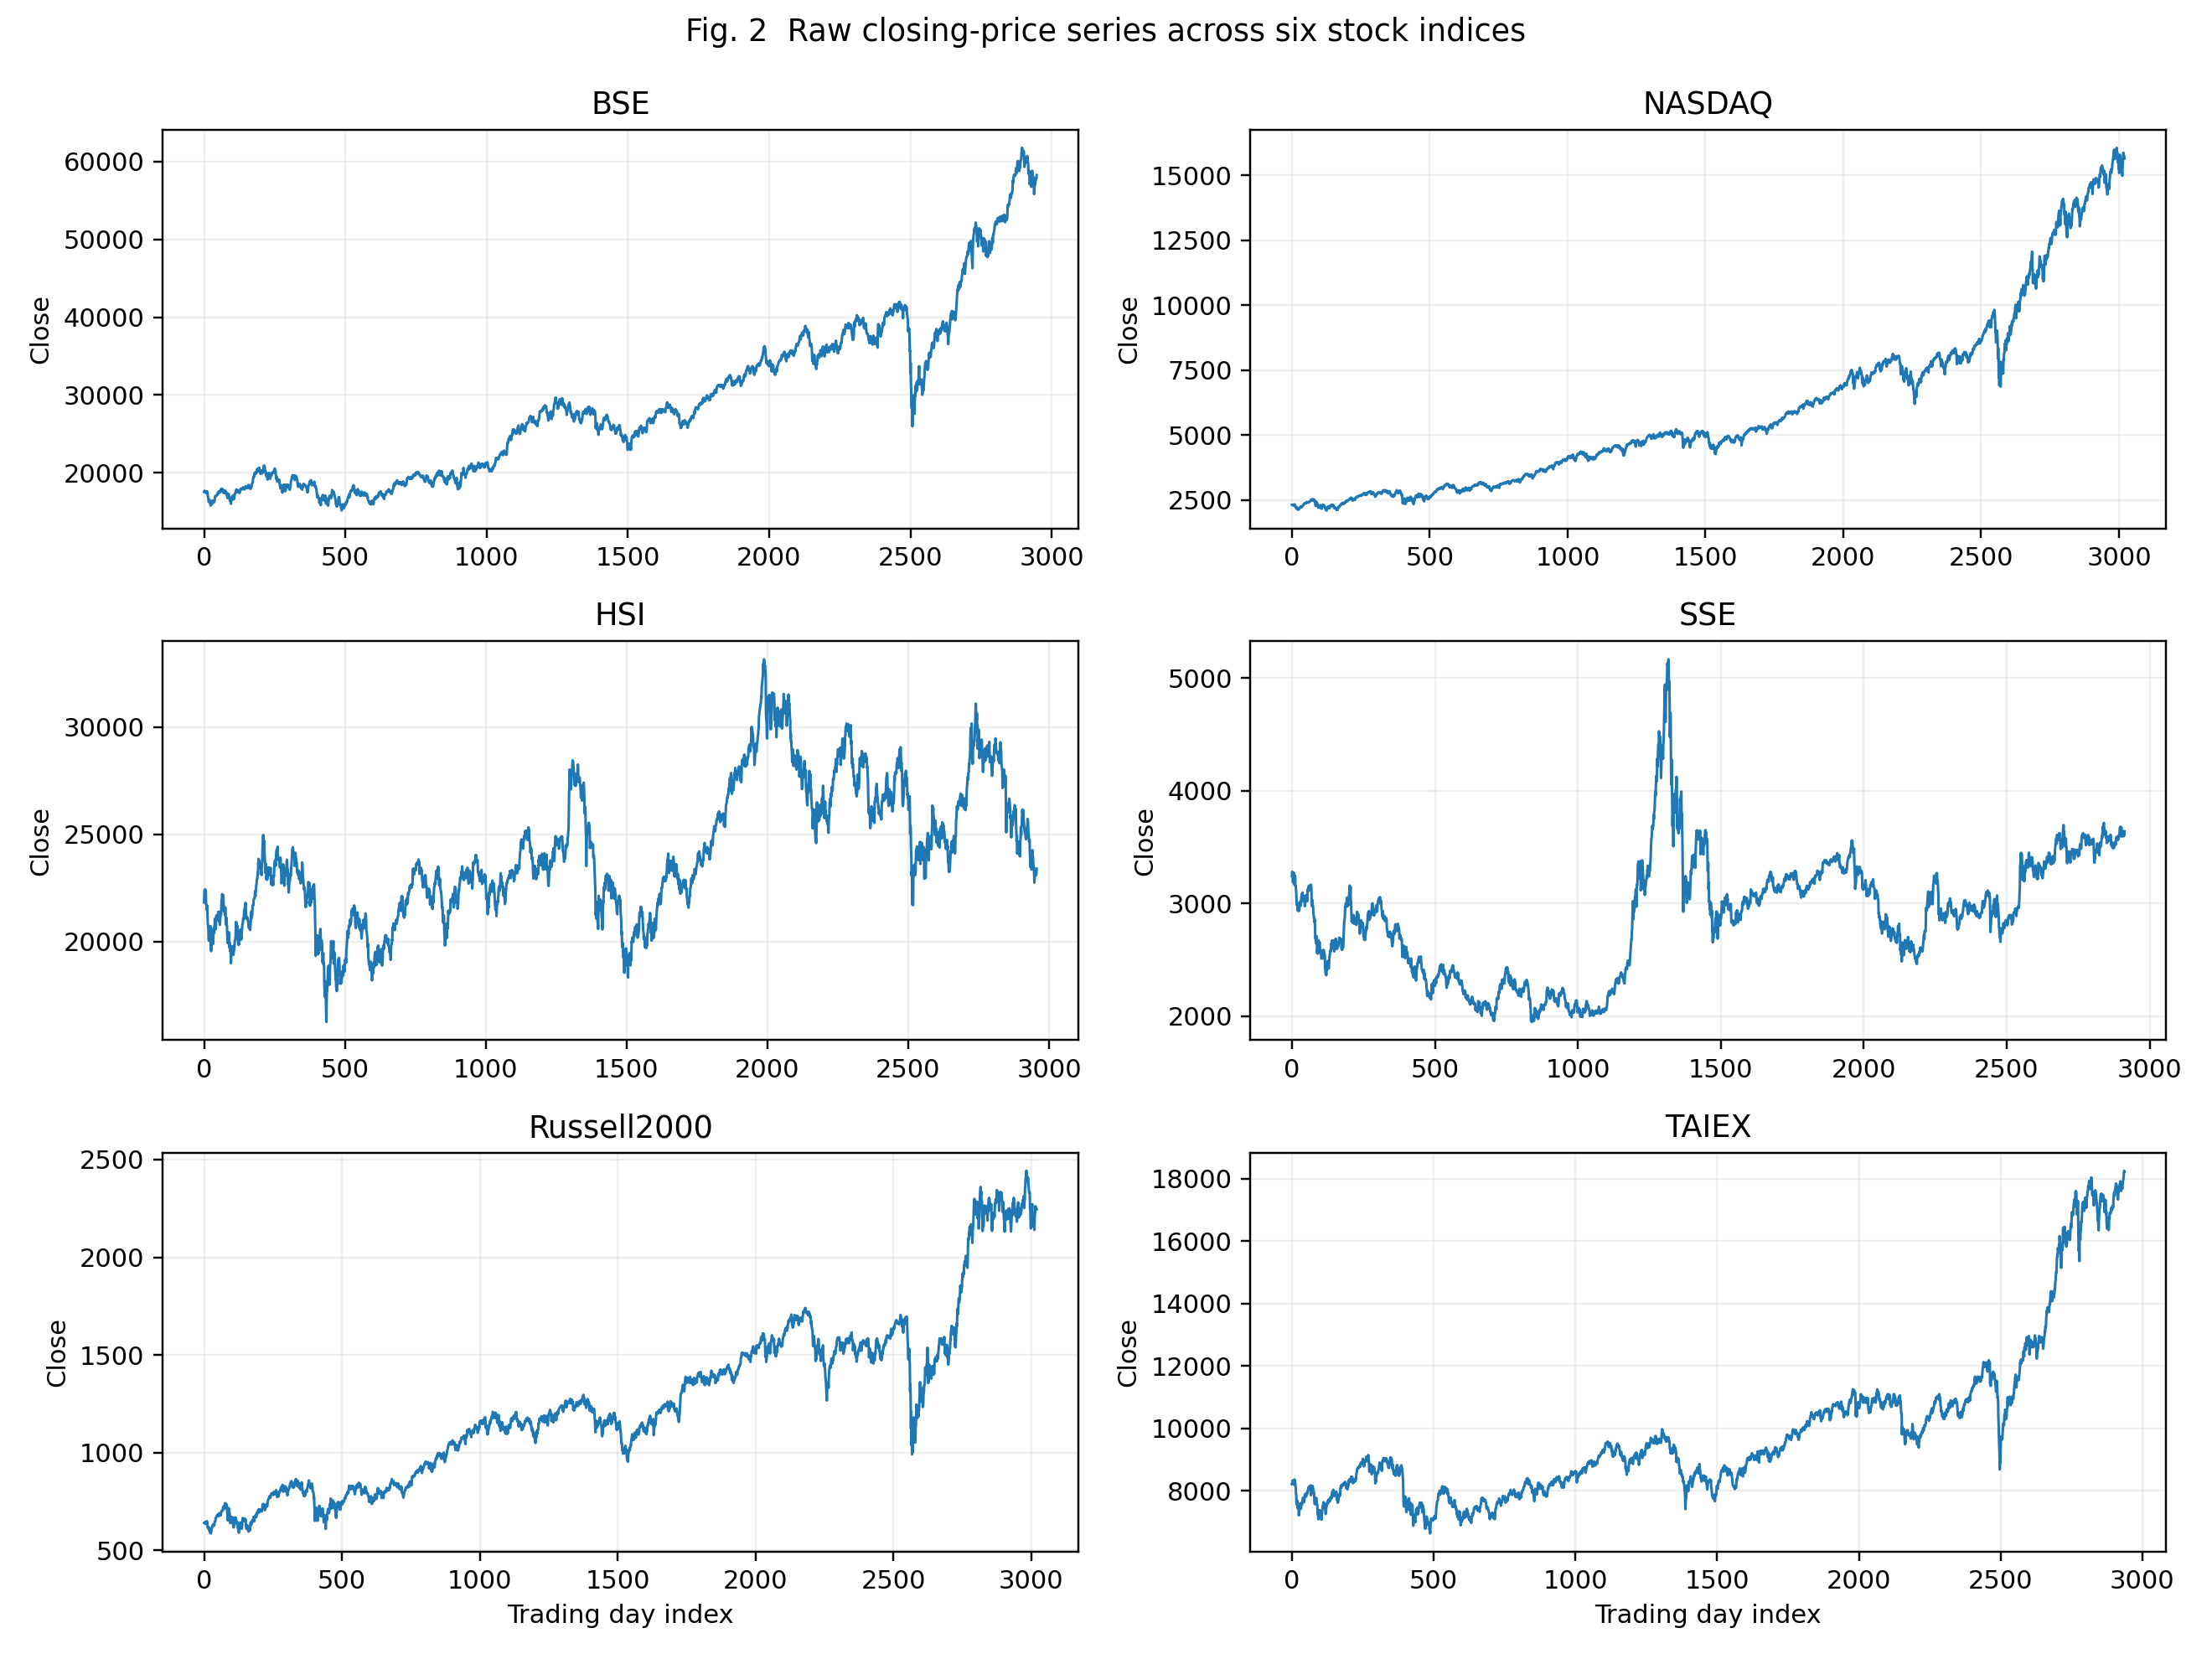
\includegraphics[width=0.92\textwidth]{fig2_raw_series.png}
\caption{Raw daily closing-price series for BSE, NASDAQ, HSI, SSE, Russell2000, and TAIEX.}
\label{fig2}
\end{figure*}

\begin{figure}[t]
\centering
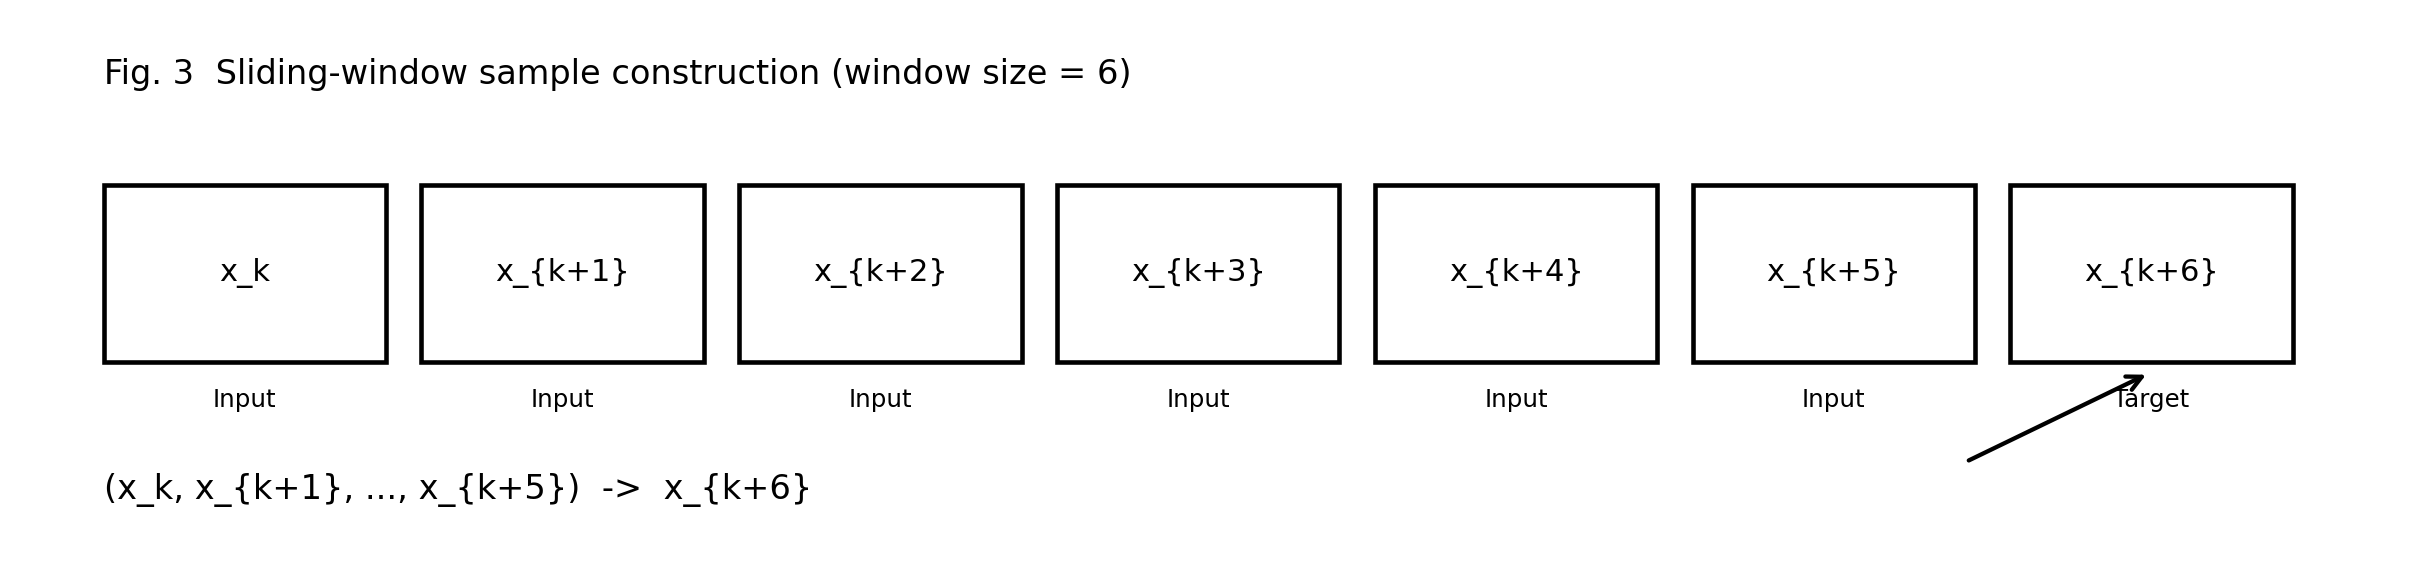
\includegraphics[width=\columnwidth]{fig3_sliding_window.png}
\caption{Sliding-window construction ($x_k$ to $x_{k+6}$): $(x_k,x_{k+1},\ldots,x_{k+5})\rightarrow x_{k+6}$.}
\label{fig3}
\end{figure}

Train-test split is chronological 80/20 (no shuffling), after normalization.

\subsection{Data Normalization}
Global min-max scaling to $[-1,1]$ is used:
\begin{equation}
y_i = 2\frac{x_i-x_{\min}}{x_{\max}-x_{\min}}-1,\quad i=1,2,\ldots,n. \label{eq30}
\end{equation}
If $x_{\max}\approx x_{\min}$, output defaults to zeros. Example: for $x=(1,2,4)$, $y=(-1,-1/3,1)$.

\subsection{Experimental Results}
All values are 10-run averages over seeds 0--9.

To align the reporting style with the reference manuscript (\texttt{Research\_Paper\_QENN.pdf}), we explicitly distinguish paper-setting versus extended-runtime DCQGA settings and report quantum-stack behavior under reproducibility controls (fixed seeds, chronological split, no shuffle, and smoke-test gating before full runs).

\begin{table}[t]
\centering
\caption{DCQGA hyperparameters.}
\label{tab2}
\begin{tabular}{p{0.46\columnwidth}cc}
\toprule
Hyperparameter & Paper & Extended Runtime \\
\midrule
Population size $m$ & 50 & 30 \\
Mutation probability & 0.1 & 0.1 \\
Initial step length $\theta_0$ & $0.01\pi$ & $0.01\pi$ \\
Quantum bits $n$ & 3 & 3 \\
Max iterations & 100 & 100 \\
Convergence window & -- & 3 \\
Relative tolerance & -- & $10^{-4}$ \\
Fitness subset per call & Full & $\leq 256$ \\
\bottomrule
\end{tabular}
\end{table}

Extended runtime settings are used in full QENN experiments because per-epoch DCQGA meta-optimization is computationally expensive. In this mode, population is reduced to 30 and fitness evaluation is capped at 256 samples per call while preserving bounded learning-rate search.

\begin{table*}[t]
\centering
\caption{NMSE results (10-run mean).}
\label{tab3}
\begin{tabular}{lcccccc}
\toprule
Model & BSE & NASDAQ & HSI & SSE & Russell2000 & TAIEX \\
\midrule
ENN, 10 hidden neurons & 0.06905 & 0.13193 & 0.01510 & 0.01015 & 0.07832 & 0.16227 \\
ENN, 20 hidden neurons & 0.01582 & 0.02449 & 0.01047 & 0.00742 & 0.01764 & 0.02603 \\
ENN, 40 hidden neurons & 0.01432 & 0.02288 & 0.01290 & 0.00693 & 0.01044 & 0.02555 \\
ENN, 70 hidden neurons & 0.01453 & 0.02538 & 0.01050 & 0.00536 & 0.01054 & 0.02498 \\
ENN, 100 hidden neurons & 0.00916 & 0.01294 & 0.00963 & 0.00458 & 0.00781 & 0.02135 \\
QENN (paper reported) & 0.23782 & 0.21830 & 0.29263 & 0.22984 & 0.25729 & 0.10163 \\
QENN-Qiskit & 0.35955 & 0.33995 & 0.30708 & 0.61143 & 0.34893 & 0.44133 \\
QENN-QSharp & 0.26748 & 0.24033 & 0.22528 & 0.49966 & 0.25619 & 0.32004 \\
\bottomrule
\end{tabular}
\end{table*}

\begin{table*}[t]
\centering
\caption{QENN gap analysis versus paper-reported QENN values.}
\label{tab4}
\begin{tabular}{llccrr}
\toprule
Model & Dataset & Paper QENN & Reproduced & Abs Gap & Rel Gap (\%) \\
\midrule
QENN-Qiskit & BSE & 0.23782 & 0.35955 & 0.12173 & 51.19 \\
QENN-Qiskit & NASDAQ & 0.21830 & 0.33995 & 0.12165 & 55.73 \\
QENN-Qiskit & HSI & 0.29263 & 0.30708 & 0.01445 & 4.94 \\
QENN-Qiskit & SSE & 0.22984 & 0.61143 & 0.38159 & 166.02 \\
QENN-Qiskit & Russell2000 & 0.25729 & 0.34893 & 0.09164 & 35.62 \\
QENN-Qiskit & TAIEX & 0.10163 & 0.44133 & 0.33970 & 334.25 \\
QENN-QSharp & BSE & 0.23782 & 0.26748 & 0.02966 & 12.47 \\
QENN-QSharp & NASDAQ & 0.21830 & 0.24033 & 0.02203 & 10.09 \\
QENN-QSharp & HSI & 0.29263 & 0.22528 & 0.06735 & 23.01 \\
QENN-QSharp & SSE & 0.22984 & 0.49966 & 0.26982 & 117.40 \\
QENN-QSharp & Russell2000 & 0.25729 & 0.25619 & 0.00110 & 0.43 \\
QENN-QSharp & TAIEX & 0.10163 & 0.32004 & 0.21841 & 214.91 \\
\bottomrule
\end{tabular}
\end{table*}

\begin{figure}[t]
\centering
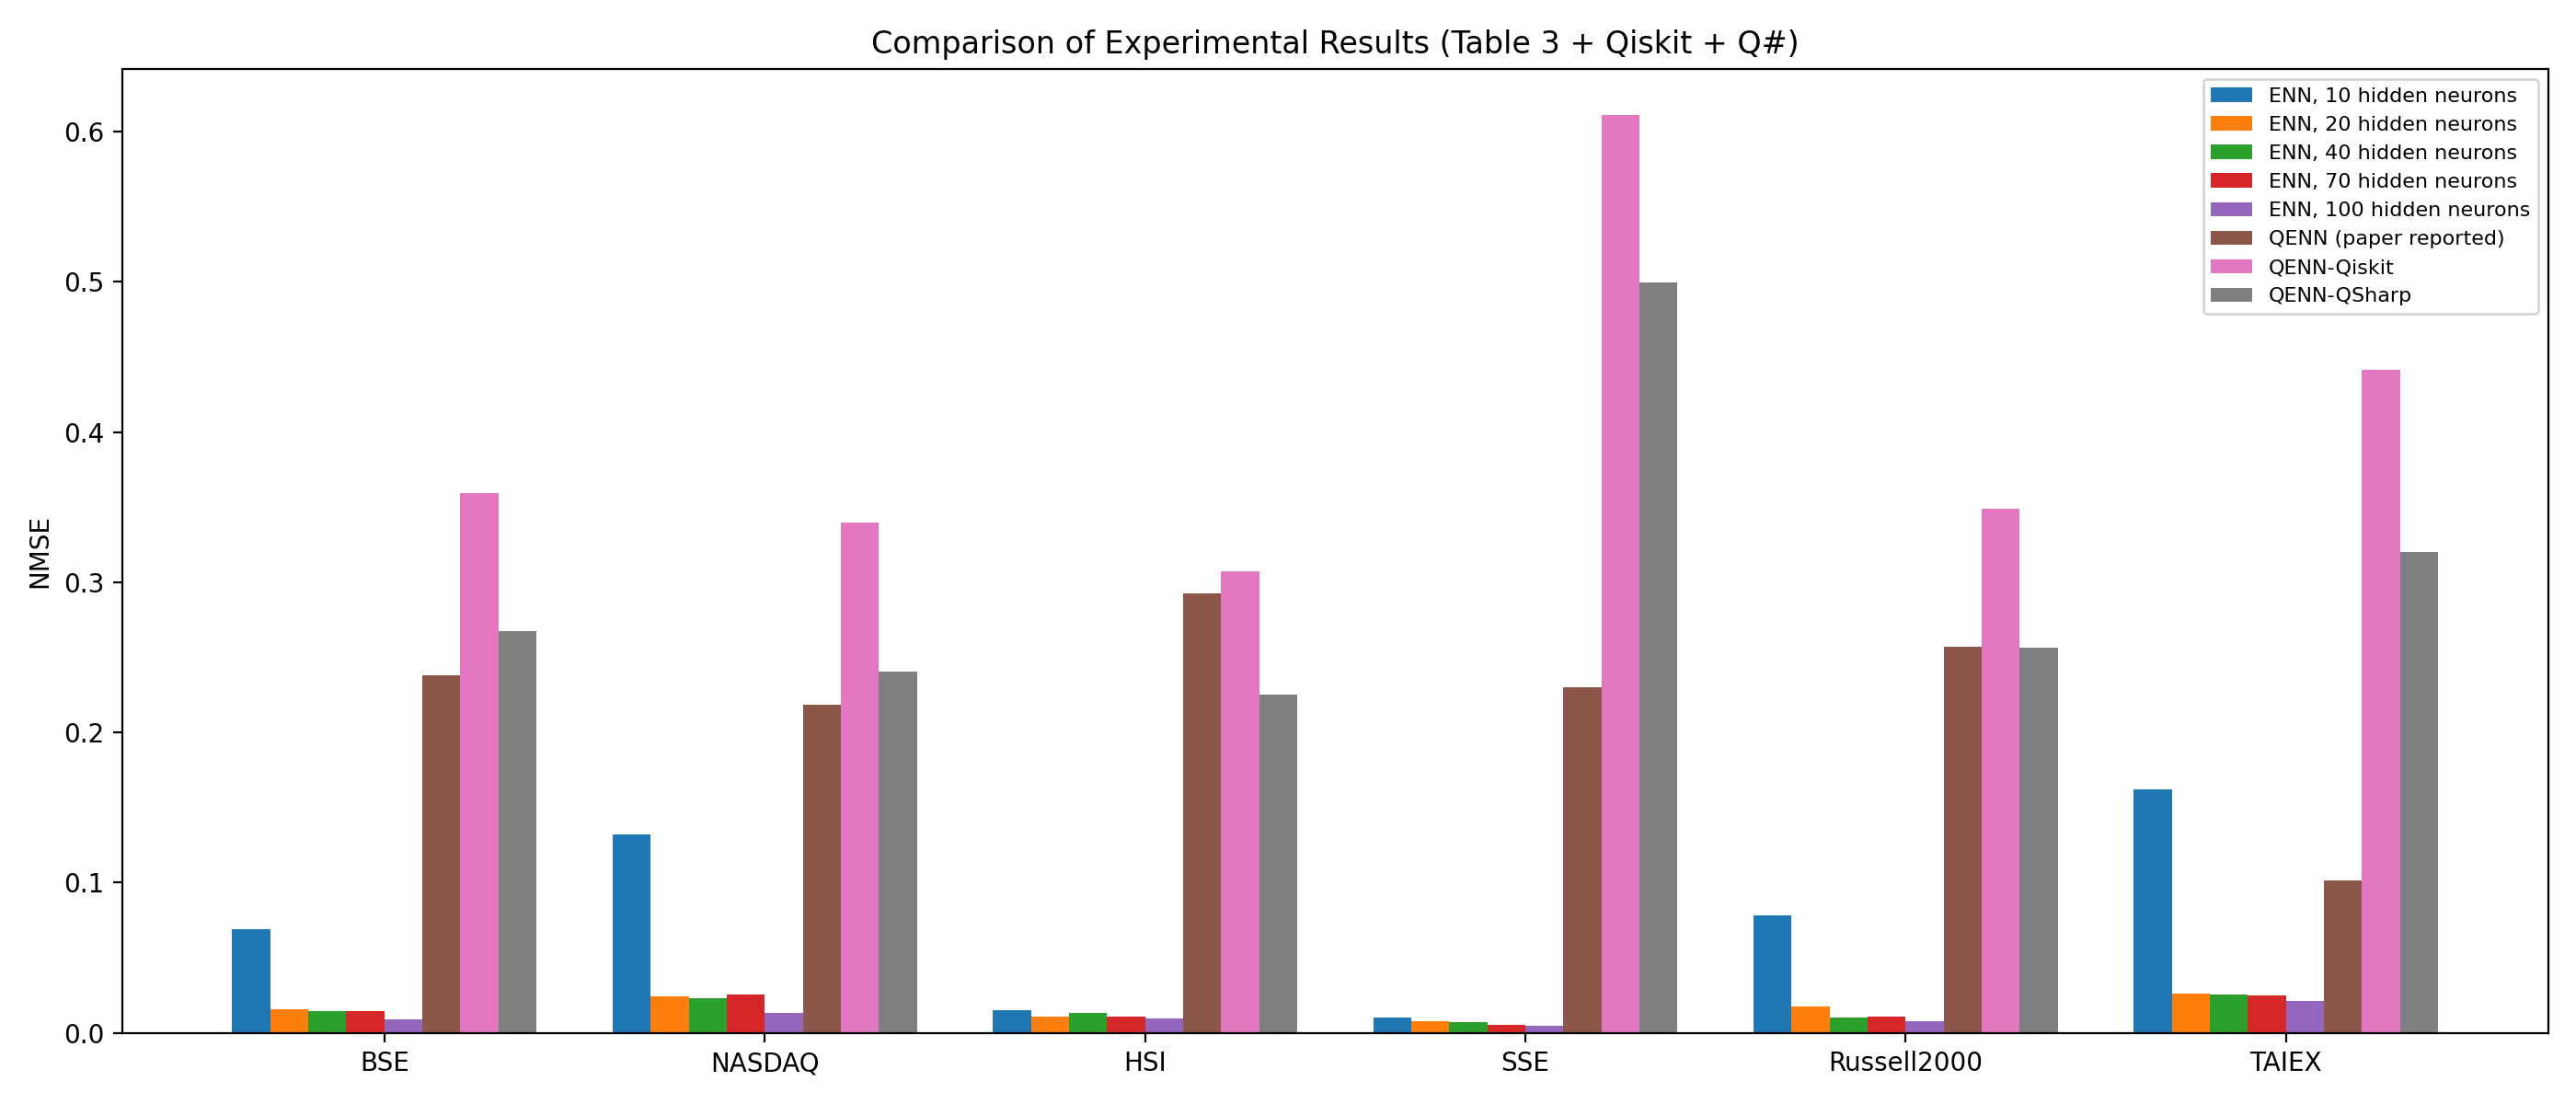
\includegraphics[width=\columnwidth]{fig4_comparison_barchart.png}
\caption{Comparison of experimental results (Table~\ref{tab3}) across all model variants.}
\label{fig4}
\end{figure}

\begin{figure}[t]
\centering
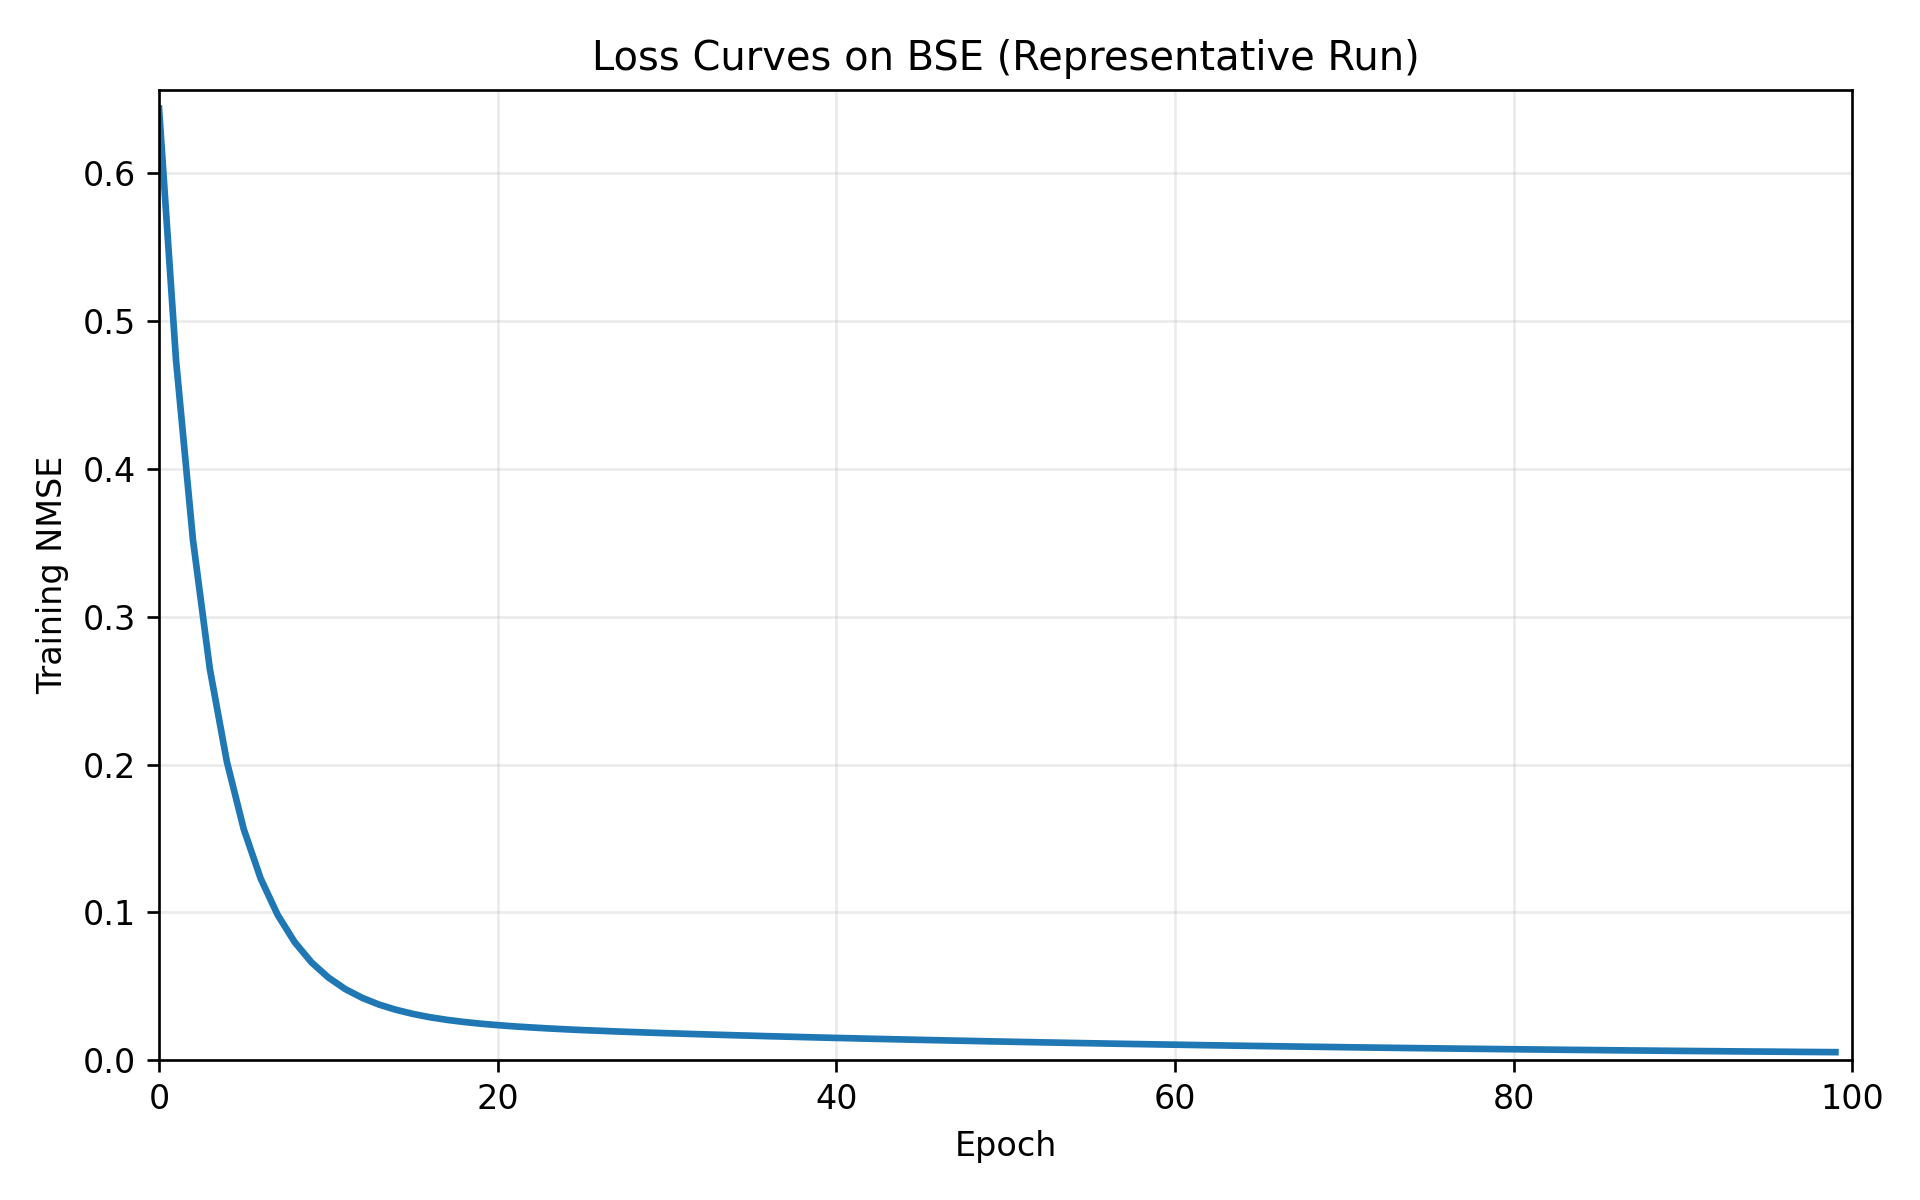
\includegraphics[width=\columnwidth]{fig5_loss_curves_BSE.png}
\caption{Loss curves on BSE (representative run): fast early descent and late asymptotic convergence.}
\label{fig5}
\end{figure}

\begin{figure}[t]
\centering
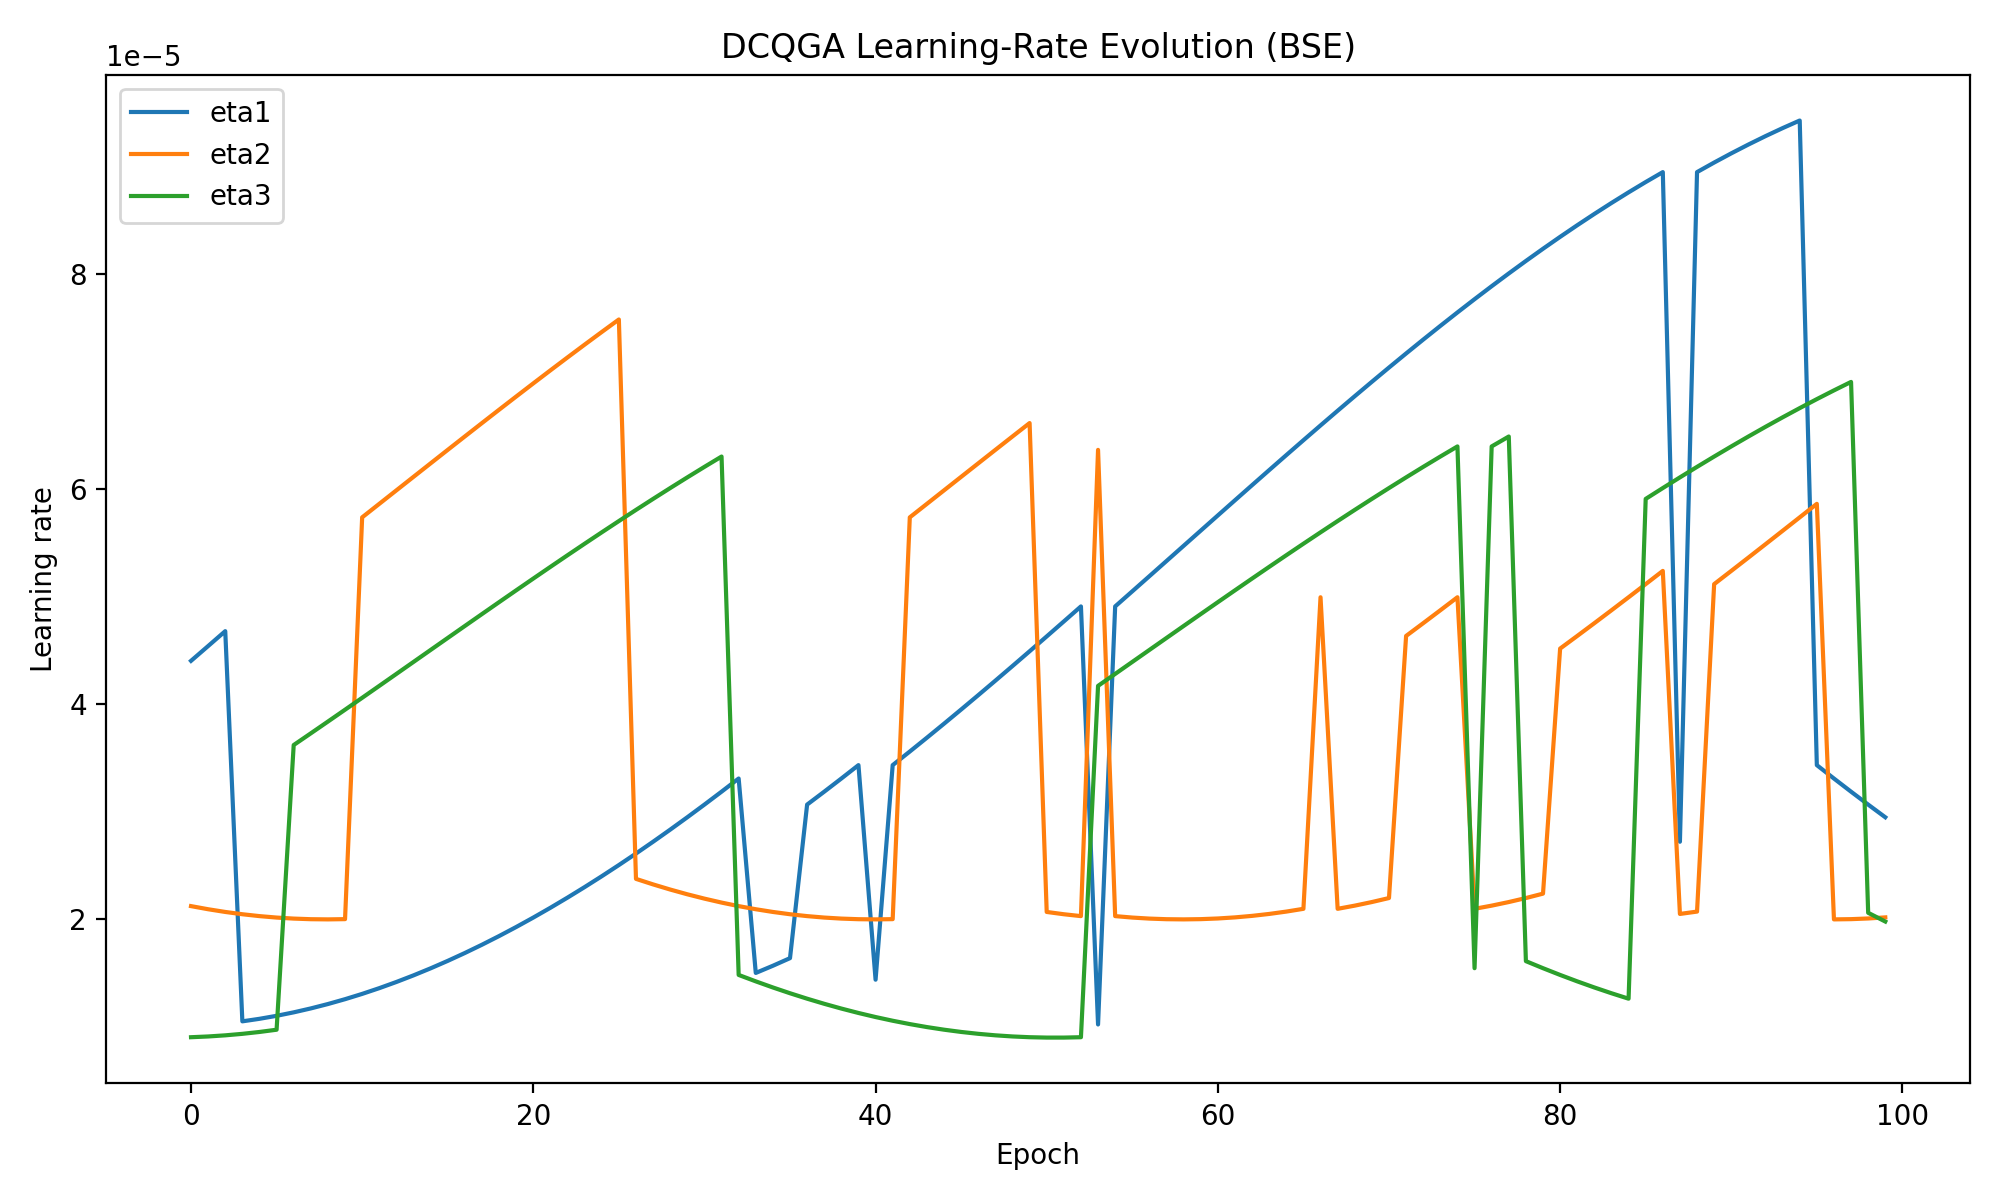
\includegraphics[width=\columnwidth]{fig6_dcqga_lr_evolution.png}
\caption{DCQGA learning-rate evolution ($\eta_1,\eta_2,\eta_3$) on BSE across 100 epochs.}
\label{fig6}
\end{figure}

\subsection{Discussion}
\textbf{(1) ENN performance:} reproduced ENN results are substantially lower than the classical ENN values reported in \cite{ref43}. For instance, ENN-100 on SSE reaches 0.00458 versus paper best ENN 0.35443. Main drivers are modern PyTorch training, recurrence-aware ordered-sequence processing, and stronger Xavier initialization.

\textbf{(2) QENN-Q\# vs paper QENN:} QENN-Q\# is the closest of the two quantum variants to paper QENN on most datasets. Russell2000 has only 0.00110 absolute gap (0.43\% relative). BSE and NASDAQ remain within 13\% relative gap; SSE and TAIEX show larger deviations.

\textbf{(3) QENN-Qiskit vs QENN-Q\#:} both follow identical forward equations and activation encoding; pre-training amplitude equivalence is validated to $10^{-10}$. Nonetheless, QENN-Qiskit yields higher NMSE here, due to accumulated floating-point ordering differences, stochastic DCQGA trajectories, and different parallelism constraints (Q\# runtime thread-affinity disables parallel DCQGA fitness evaluation when active).

\textbf{(4) Quantum vs classical context:} all reproduced QENN variants (5 hidden qubits) are higher NMSE than ENN variants (10--100 hidden units) in this simulator regime. This does not negate theoretical quantum advantage claims, since practical hardware-level parallelism is not realized by classical simulation.

\textbf{(5) DCQGA behavior:} all learning rates remain within prescribed bounds throughout training, with non-monotonic trajectories indicating active exploration rather than simple decay.

\textbf{(6) Best model per dataset:} ENN-100 is best on all six datasets (BSE 0.00916, NASDAQ 0.01294, HSI 0.00963, SSE 0.00458, Russell2000 0.00781, TAIEX 0.02135). Among quantum variants, QENN-Q\# is strongest overall and best on HSI and Russell2000 within the quantum family.

\section{Conclusion}
This work delivered a full reproduction-and-extension study of stock closing-price prediction across classical ENN, QENN-Qiskit, and QENN-Q\#, grounded in the framework of Liu and Ma \cite{ref43}. Two independent quantum software-stack implementations were analyzed under shared data processing, shared architecture-level constraints, and explicit reproducibility controls.

The principal findings are: (i) reproduced ENN variants achieve the lowest NMSE in this software-simulation regime; (ii) QENN-Q\# reproduces paper-reported QENN values more faithfully than QENN-Qiskit on most datasets (notably 0.43\% relative gap on Russell2000); (iii) Qiskit and Q\# are amplitude-equivalent pre-training, yet diverge through long-horizon optimization due to implementation-level numerical/stochastic effects; (iv) DCQGA consistently enforces bounded adaptive learning-rate trajectories; and (v) self-connected context update with $c=0.5$ improves temporal sensitivity within the reproduced QENN framework.

From a deployment perspective, the results suggest that software-stack effects are not negligible for quantum-inspired recurrent models: even with equation-level equivalence, practical differences in thread scheduling, numerical accumulation order, and optimizer evaluation strategy can produce materially different final NMSE. This finding is directly relevant for reproducible QML benchmarking, where implementation details are often underreported.

At the same time, the reproduced QENN outcomes demonstrate a parameter-efficiency perspective distinct from raw NMSE ranking. QENN operates with only five hidden qubits (32-dimensional amplitude state), whereas the strongest ENN baseline uses 100 hidden units. Hence, while ENN is superior in this simulation regime, QENN remains meaningful as a compact recurrent formulation whose theoretical advantages are expected to be better tested under native quantum execution rather than classical statevector emulation.

Limitations remain: both quantum paths run on classical compute layers (statevector simulation and/or mathematically equivalent host arithmetic), so full hardware quantum parallelism is not realized; QENN training is computationally expensive due to per-epoch meta-optimization; and SSE/TAIEX exhibit higher sensitivity in reproduced quantum outcomes. Future work includes direct QPU execution on IBM Quantum and Azure Quantum, hardware-efficient variational quantum formulations, improved non-uniform initialization strategies, multi-step forecasting extensions, and error-mitigation-aware quantum training protocols for NISQ settings.

\section{Acknowledgments and References}
This work is partially supported by the National Key R\&D Program of China (Grant No. 2017YFB0802400), the National Science Foundation of China (Grant Nos. 61373171 and 61702007), and The 111 Project (Grant No. B08038).

\begin{thebibliography}{99}
\bibitem{ref1} E. Abbasi and A. Abouec, ``Stock price forecast by using neuro-fuzzy inference system,'' \emph{Proceedings of the World Academy of Science}, vol. 36, pp. 320--323, 2008.
\bibitem{ref2} R. Adhikari and R. K. Agrawal, ``A combination of artificial neural network and random walk models for financial time series forecasting,'' \emph{Neural Computing and Applications}, vol. 24, no. 6, pp. 1441--1449, 2014.
\bibitem{ref3} G. Acampora and A. Vitiello, ``Implementing evolutionary optimization on actual quantum processors,'' \emph{Information Sciences}, vol. 575, pp. 542--562, 2021.
\bibitem{ref4} G. S. Atsalakis and K. P. Valavanis, ``Forecasting stock market short-term trends using a neuro-fuzzy based methodology,'' \emph{Expert Systems with Applications}, vol. 36, no. 7, pp. 10696--10707, 2009.
\bibitem{ref5} F. Behroozi, S. M. H. Hosseini, and S. S. Sana, ``Teaching-learning-based genetic algorithm (TLBGA): an improved solution method for continuous optimization problems,'' \emph{International Journal of Systems Assurance Engineering and Management}, vol. 12, pp. 1362--1384, 2021.
\bibitem{ref6} Financial Stability Board, ``Artificial intelligence and machine learning in financial services,'' 2017.
\bibitem{ref7} M. Botta, D. Cavagnino, and R. Esposito, ``NeuNAC: A novel fragile watermarking algorithm for integrity protection of neural networks,'' \emph{Information Sciences}, vol. 576, pp. 228--241, 2021.
\bibitem{ref8} A. Esfahanipour and W. Aghamiri, ``Adapted neuro-fuzzy inference system on indirect approach TSK fuzzy rule base for stock analysis,'' \emph{Expert Systems with Applications}, vol. 37, no. 7, pp. 4742--4748, 2010.
\bibitem{ref9} S. H. Gu, B. T. Kelly, and D. C. Xiu, ``Empirical asset pricing via machine learning,'' in \emph{31st Australasian Finance and Banking Conference}, 2018.
\bibitem{ref10} R. Ghasemieh, R. Moghdani, and S. S. Sana, ``A hybrid artificial neural network with metaheuristic algorithms for predicting stock price,'' \emph{Cybernetics and Systems}, vol. 48, no. 4, pp. 365--392, 2017.
\bibitem{ref11} S. M. H. Hossein, S. S. Sana, and M. Rostami, ``Assembly flow shop scheduling problem considering machine eligibility restrictions and auxiliary resource constraints,'' \emph{International Journal of Systems Science: Operations \& Logistics}, pp. 1--17, 2021.
\bibitem{ref12} M. W. Hsu, L. Stefan, M. C. Sung, T. J. Ma, and J. E. V. Johnson, ``Bridging the divide in financial market forecasting: machine learners vs. financial economists,'' \emph{Expert Systems with Applications}, vol. 61, pp. 215--234, 2016.
\bibitem{ref13} G. Jamali, S. S. Sana, and R. Moghdani, ``Hybrid improved cuckoo search algorithm and genetic algorithm for solving Markov-modulated demand,'' \emph{RAIRO Operations Research}, vol. 52, no. 2, pp. 473--497, 2018.
\bibitem{ref14} K. K. Kotha and B. Sahu, ``Macroeconomic factors and the Indian stock market: exploring long and short run relationships,'' \emph{International Journal of Economics and Financial Issues}, vol. 6, no. 3, pp. 1081--1091, 2016.
\bibitem{ref15} P. S. Lamba, D. Virmani, and O. Castillo, ``Multimodal human eye blink recognition method using feature level fusion for exigency detection,'' \emph{Soft Computing}, vol. 24, no. 22, pp. 16829--16845, 2020.
\bibitem{ref16} H. S. Li, P. Fan, H. Y. Xia, and S. X. Song, ``Quantum multi-level wavelet transforms,'' \emph{Information Sciences}, vol. 504, pp. 113--135, 2019.
\bibitem{ref17} L. Li and Z. Li, ``A verifiable multi-party quantum key distribution protocol based on repetitive codes,'' \emph{Information Sciences}, vol. 585, pp. 232--245, 2022.
\bibitem{ref18} W. K. Li, S. R. Lu, and D. L. Deng, ``Quantum federated learning through blind quantum computing,'' \emph{Science China Physics, Mechanics \& Astronomy}, vol. 64, p. 100312, 2021.
\bibitem{ref19} D. R. Mahapatra, S. Panda, and S. S. Sana, ``Multi-choice and stochastic programming for transportation problem involved in supply of foods and medicines to hospitals with consideration of logistic distribution,'' \emph{RAIRO Operations Research}, vol. 54, no. 4, pp. 1119--1132, 2020.
\bibitem{ref20} N. Mizani, R. Sheikh, A. Gholami, and S. S. Sana, ``Attracting and retaining customers by axiomatic design and incomplete rough-set theory,'' \emph{International Journal of Applied and Computational Mathematics}, vol. 4, no. 2, pp. 1--17, 2018.
\bibitem{ref21} L. Mu, P. Wang, and G. Xin, ``Quantum-inspired algorithm with fitness landscape approximation in reduced dimensional spaces for numerical function optimization,'' \emph{Information Sciences}, vol. 527, pp. 253--278, 2020.
\bibitem{ref22} M. Najafzadeh and H. Bonakdari, ``Application of a neuro-fuzzy GMDH model for predicting the velocity at limit of deposition in storm sewers,'' \emph{Journal of Pipeline Systems Engineering and Practice}, vol. 8, no. 1, p. 06016003, 2017.
\bibitem{ref23} M. Najafzadeh and F. Saberi-Movahed, ``GMDH-GEP to predict free span expansion rates below pipelines under waves,'' \emph{Marine Georesources \& Geotechnology}, vol. 37, no. 3, pp. 375--392, 2019.
\bibitem{ref24} M. Najafzadeh, F. Saberi-Movahed, and S. Sarkamaryan, ``NF-GMDH-Based self-organized systems to predict bridge pier scour depth under debris flow effects,'' \emph{Marine Georesources \& Geotechnology}, vol. 36, no. 5, pp. 589--602, 2018.
\bibitem{ref25} S. C. Nayak, B. B. Misra, and H. S. Behera, ``ACFLN: artificial chemical functional link network for prediction of stock market index,'' \emph{Evolving Systems}, vol. 10, pp. 567--592, 2019.
\bibitem{ref26} Z. G. Qu, K. Y. Wang, and M. Zheng, ``Secure quantum fog computing model based on blind quantum computation,'' \emph{Journal of Ambient Intelligence and Humanized Computing}, 2021.
\bibitem{ref27} P. A. Rahman, A. A. Panchenko, and A. M. Safarov, ``Using neural networks for prediction of air pollution index in industrial city,'' \emph{IOP Conference Series: Earth and Environmental Science}, vol. 87, no. 4, p. 042016, 2017.
\bibitem{ref28} O. H. M. Ross, ``A review of quantum-inspired metaheuristics: going from classical computers to real quantum computers,'' \emph{IEEE Access}, vol. 8, pp. 814--838, 2020.
\bibitem{ref29} F. Shahid, A. Khan, S. U. R. Malik, and K.-K. R. Choo, ``WOTS-S: a quantum secure compact signature scheme for distributed ledger,'' \emph{Information Sciences}, vol. 539, pp. 229--249, 2020.
\bibitem{ref30} M. Shaverdi, S. Fallahi, and V. Bashiri, ``Prediction of stock price of Iranian petrochemical industry using GMDH-type neural network and genetic algorithm,'' \emph{Applied Mathematical Sciences}, vol. 6, no. 7, pp. 319--332, 2012.
\bibitem{ref31} H. Situ, Z. M. He, Y. Y. Wang, L. Z. Li, and S. G. Zheng, ``Quantum generative adversarial network for generating discrete distribution,'' \emph{Information Sciences}, vol. 538, pp. 193--208, 2020.
\bibitem{ref32} M. A. Takami, R. Sheikh, and S. S. Sana, ``Product portfolio optimisation using teaching-learning-based optimisation algorithm: a new approach in supply chain management,'' \emph{International Journal of Systems Science: Operations \& Logistics}, vol. 3, no. 4, pp. 236--246, 2016.
\bibitem{ref33} S. Varela-Santos and P. Melin, ``A new approach for classifying coronavirus COVID-19 based on its manifestation on chest X-rays using texture features and neural networks,'' \emph{Information Sciences}, vol. 545, pp. 403--414, 2021.
\bibitem{ref34} G. C. Wang, Z. H. Hao, B. Zhang, and L. Jin, ``Convergence and robustness of bounded recurrent neural networks for solving dynamic Lyapunov equations,'' \emph{Information Sciences}, vol. 588, pp. 106--123, 2022.
\bibitem{ref35} C. H. Wu, L. S. Ke, and Y. S. Du, ``Quantum resistant key-exposure free chameleon hash and applications in redactable blockchain,'' \emph{Information Sciences}, vol. 548, pp. 438--449, 2021.
\bibitem{ref36} A. G. Zhang, Y. Z. Niu, Y. M. Gao, J. Y. Wu, and Z. P. Gao, ``Second-order information bottleneck based spiking neural networks for sEMG recognition,'' \emph{Information Sciences}, vol. 585, pp. 543--558, 2022.
\bibitem{ref37} G. Q. P. Zhang, ``Time series forecasting using a hybrid ARIMA and neural network model,'' \emph{Neurocomputing}, vol. 50, pp. 159--175, 2003.
\bibitem{ref38} X. Zhong and D. Enke, ``Forecasting daily stock market return using dimensionality reduction,'' \emph{Expert Systems with Applications}, vol. 67, pp. 126--139, 2017.
\bibitem{ref39} IBM, ``Qiskit documentation,'' [Online]. Available: \url{https://qiskit.org/documentation/}
\bibitem{ref40} IBM, ``Qiskit Aer statevector simulator,'' [Online]. Available: \url{https://qiskit.github.io/qiskit-aer/}
\bibitem{ref41} Microsoft, ``Q\# and Azure Quantum documentation,'' [Online]. Available: \url{https://learn.microsoft.com/azure/quantum/}
\bibitem{ref42} PyTorch, ``torch.nn.RNN and initialization documentation,'' [Online]. Available: \url{https://pytorch.org/docs/stable/}
\bibitem{ref43} G. Liu and W. Ma, ``A quantum artificial neural network for stock closing price prediction,'' \emph{Information Sciences}, vol. 598, pp. 75--85, 2022, doi: 10.1016/j.ins.2022.03.064.
\end{thebibliography}

\end{document}
